\documentclass{anstrans}
%%%%%%%%%%%%%%%%%%%%%%%%%%%%%%%%%%%
\title{MHTGR-350 Moltres Benchmark}
\author{Roberto E. Fairhurst Agosta, Kathryn D. Huff}

\institute{
University of Illinois at Urbana-Champaign, Dept. of Nuclear, Plasma, and Radiological Engineering\\
ref3@illinois.edu
}

%%%% packages and definitions (optional)
\usepackage{graphicx} % allows inclusion of graphics
\usepackage{booktabs} % nice rules (thick lines) for tables
\usepackage{microtype} % improves typography for PDF
\usepackage{xspace}
\usepackage{tabularx}
\usepackage{floatrow}
\usepackage{subcaption}
\usepackage{enumitem}
\usepackage{placeins}
\usepackage{amsmath}
\usepackage[acronym,toc]{glossaries}
\newacronym{CR}{CR}{control rod}
\newacronym{EOEC}{EOEC}{end of equilibrium cycle}
\newacronym{FDM}{FDM}{Finite Difference Method}
\newacronym{FEM}{FEM}{Finite Element Method}
\newacronym{GRS}{GRS}{Gesellschaft für Anlagen und Reaktorsicherheit}
\newacronym{He}{He}{helium}
\newacronym{HZDR}{HZDR}{Helmholtz-Zentrum Dresden-Rossendorf}
\newacronym{HTGR}{HTGR}{High Temperature Gas-Cooled Reactor}
\newacronym{HTR}{HTR}{High Temperature Reactor}
\newacronym{HTTR}{HTTR}{High Temperature Test Reactor}
\newacronym{IPyC}{IPyC}{inner pyrolitic carbon}
\newacronym{INL}{INL}{Idaho National Laboratory}
\newacronym{KAERI}{KAERI}{Korea Atomic Energy Research Institute}
\newacronym{LWR}{LWR}{Light Water Reactor}
\newacronym{MC}{MC}{Monte Carlo}
\newacronym{MHTGR}{MHTGR}{Modular High-Temperature Gas-Cooled Reactor}
\newacronym{MOOSE}{MOOSE}{Multiphysics Object-Oriented Simulation Environment}
\newacronym{MSR}{MSR}{Molten Salt Reactor}
\newacronym{NEA}{NEA}{Nuclear Energy Agency}
\newacronym{NEM}{NEM}{Nodal Expansion Method}
\newacronym{NRC}{NRC}{Nuclear Regulatory Commission}
\newacronym{NSC}{NSC}{Nuclear Science Committee}
\newacronym{OECD}{OECD}{Organisation for Economic Co-operation and Development}
\newacronym{OPyC}{OPyC}{outer pyrolitic carbon}
\newacronym{PBMR}{PBMR}{Pebble Bed Modular Reactor}
\newacronym{PMR}{PMR}{Prismatic Modular Reactor}
\newacronym{RSD}{RSD}{Relative Standard Deviation}
\newacronym{SD}{SD}{Standard Deviation}
\newacronym{SiC}{SiC}{silicon carbide}
\newacronym{SNU}{SNU}{Seoul National University}
\newacronym{TRISO}{TRISO}{Tristructural Isotropic}
\newacronym{UIUC}{UIUC}{University of Illinois at Urbana-Champaign}
\newacronym{UNIST}{UNIST}{Ulsan National Intitute of Science and Technology}
\newacronym{UK}{UK}{United Kingdom}
\newacronym{UMICH}{UMICH}{Universtiy of Michigan}
\newacronym{US}{US}{United States}
\newacronym{VHTR}{VHTR}{very high temperature reactor}
%\newacronym{<++>}{<++>}{<++>}
%\newacronym{<++>}{<++>}{<++>}

\makeglossaries

\usepackage[printwatermark]{xwatermark}
\usepackage{xcolor}
\usepackage{graphicx}
\usepackage{lipsum}

\newcommand{\SN}{S$_N$}
\renewcommand{\vec}[1]{\bm{#1}} %vector is bold italic
\newcommand{\vd}{\bm{\cdot}} % slightly bold vector dot
\newcommand{\grad}{\vec{\nabla}} % gradient
\newcommand{\ud}{\mathop{}\!\mathrm{d}} % upright derivative symbol

\newcolumntype{c}{>{\hsize=.56\hsize}X}
\newcolumntype{b}{>{\hsize=.7\hsize}X}
\newcolumntype{s}{>{\hsize=.74\hsize}X}
\newcolumntype{f}{>{\hsize=.1\hsize}X}
\newcolumntype{a}{>{\hsize=.45\hsize}X}
%\usepackage[pagestyles]{titlesec}
%\titleformat*{\subsection}{\normalfont}
%\titleformat{\section}{\bfseries}{Item \thesection.\ }{0pt}{}

%\newwatermark[allpages,color=gray!50,angle=45,scale=3,xpos=0,ypos=0]{DRAFT}

\begin{document}
%%%%%%%%%%%%%%%%%%%%%%%%%%%%%%%%%%%%%%%%%%%%%%%%%%%%%%%%%%%%%%%%%%%%%%%%%%%%%%%%
\section{Introduction}

The history of \glspl{PMR} begins in the 1960s with the deployment of the Dragon reactor (1965) in the \gls{UK} and Peach Bottom (1966) in the \gls{US}.
Later on, the Fort St. Vrain Generating Station (1976) in the \gls{US} laid the foundation for future prismatic \gls{HTGR} designs.
Modern \gls{HTGR} designs still use variants of its fuel assembly block.

Although the \gls{PMR} design concept have existed for some time, the deterministic neutronic thermal-fluids and transient analysis tools and methods available for the  design and analysis of \glspl{PMR} have lagged behind the state of the art compared to other reactor technologies \cite{oecd_nea_benchmark_2017}.
This has not only motivated the testing of existing methods for \glspl{HTGR} but also the development of more accurate and efficient tools for the design and safety evaluations of the \gls{PMR}.

In addition to the development of new methods, it is essential to define appropriate benchmarks to compare the capabilities of various computer codes.
The OECE \gls{NEA} defined such benchmark for the MHTGR-350 reactor \cite{oecd_nea_benchmark_2017}.
The scope of the benchmark is twofold: 1) to establish a well-defined problem, based on a common given data set, to compare methods and tools in core simulation and thermal fluids analysis, 2) to test the depletion capabilities of various lattice physics codes available for \glspl{PMR}.

The objective of this work is to conduct exercise 1 of Phase I of the benchmark with the \gls{MOOSE} \cite{gaston_physics-based_2015} based tool \textit{Moltres}\cite{lindsay_introduction_2018}.

\section{Benchmark definition}

The MHTGR-350 is a General Atomics design developed in the 1980s.
This reactor forms the base of the reference design.
The benchmark specifies the fuel at the \gls{EOEC} core state because it leads to the highest decay heat load for the system and narrowest safety margins \cite{ortensi_prismatic_2011}.

The core consists of an array of hexagonal fuel elements in a cylindrical arrangement \ref{fig:radial}.
A ring of identically sized solid graphite replaceable reflector elements surrounds the fuel elements.
Then, a region of permanent reflector elements follows the replaceable reflectors.
19 graphite replaceable reflector elements compose an inner reflector.
The RPV encases all the elements.

Figure \ref{fig:axial} shows an axial view of the reactor.
The active core consists of hexagonal graphite fuel elements containing blind holes for fuel compacts and full-length channels for helium coolant flow.
10 fuel elements stacked on top of each other compose the 66 fuel columns that integrate the active core.

Thirty reflector columns contain channels for control rods.
Twelve columns in the core also contain channels for reserve shutdown borated graphite pellets.

\begin{figure}[htbp!] %or H 
	\centering
	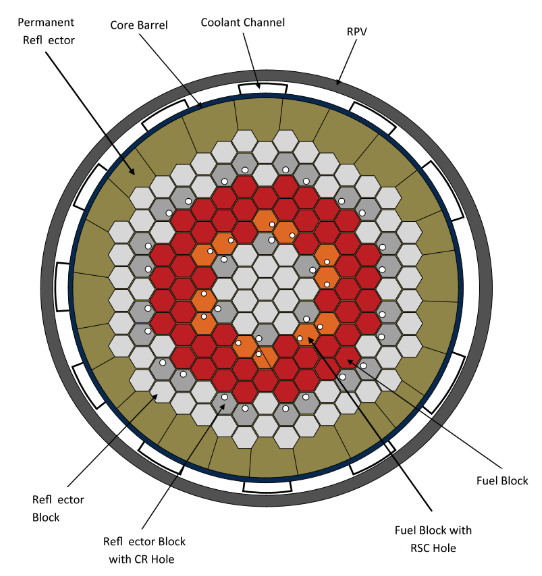
\includegraphics[width=0.95\linewidth]{figures/radial-layout.png}
	\hfill
	\caption{Core radial layout. Image reproduced from \cite{oecd_nea_benchmark_2017}.}
	\label{fig:radial}
\end{figure}

\begin{figure}[htbp!]
	\centering
	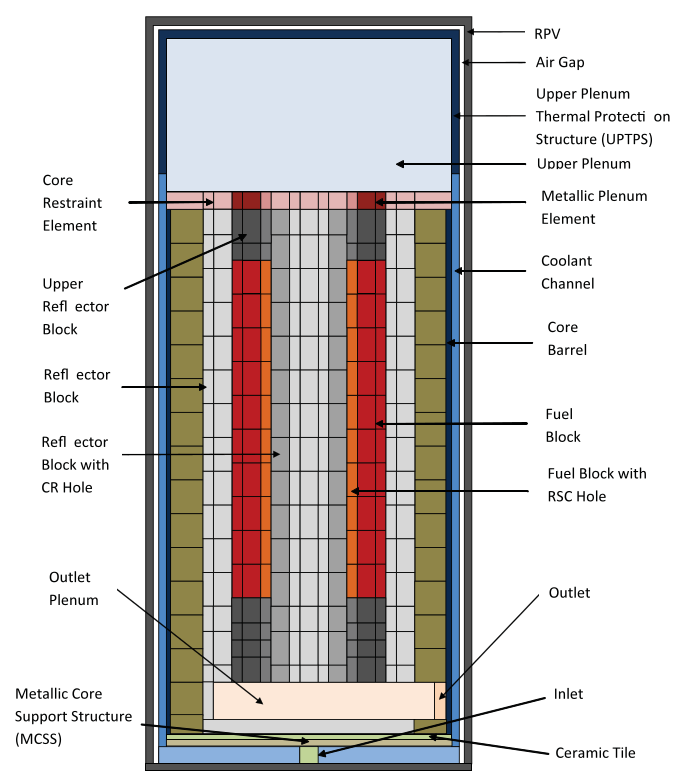
\includegraphics[width=0.95\linewidth]{figures/axial-layout.png}
	\hfill
	\caption{Core axial layout. Image reproduced from \cite{oecd_nea_benchmark_2017}.}
	\label{fig:axial}
\end{figure}

\subsection{Benchmark cases}

\begin{itemize}
	\item Phase I: Steady State
\end{itemize}

The following is a list of the proposed exercises for the steady state calculations:

\begin{enumerate}
	\item Neutronics solution with fixed cross sections. 
	\item Thermal fluids solution with given heat sources.
	\item Coupled neutronics-thermal fluids steady state solution.
\end{enumerate}

As mentioned earlier, the scope of this work is exercise 1 of Phase I.
Future studies will focus on the rest of the exercises of Phase I.

The benchmark specifies the cross sections required to conduct the exercise.
This ensures a common dataset among different benchmark participants.
The weighted multi-group macroscopic cross sections were obtained using DRAGON-4 \cite{marleau_user_2016}from a full block configuration with a double heterogeneity treatment of the fuel \cite{ortensi_prismatic_2011}.
The dataset contains 26 energy groups.

\begin{itemize}
	\item Phase II: Transient Cases
\end{itemize}

The following is a list of the proposed exercises for the transient calculations:

\begin{enumerate}
	\item Depressurized Conduction Cooldown without reactor trip.
	\item Pressurized Conduction Cooldown with reactor trip.
	\item Water ingress with reactor trip.
	\item Power 100-80-100 load follow.
\end{enumerate}

Future studies will focus on Phase II.

\begin{itemize}
	\item Phase III: Lattice Depletion Case
\end{itemize}

This phase intends to examine variations in lattice calculations.
We do not plan to conduct studies of such phase in the future.

\section{Moltres}

Moltres is an open source simulation tool originally developed for simulating \glspl{MSR} in the context of the \gls{MOOSE} finite element modeling framework.
Moltres defines physics kernels and boundary conditions that solve arbitrary-group neutron diffusion, temperature, and precursor governing equations on a single mesh from one to three dimensions.
In \gls{MOOSE} jargon, kernels are C++ classes that contain methods for computing residual and Jacobian contributions corresponding to individual pieces of governing equations \cite{lindsay_introduction_2018}.

In Moltres, the time-dependent multi-group diffusion equation, equation \ref{eq:diffusion}, describes the group $g$ neutron flux.

\begin{align}
        \frac{1}{v_g}\frac{\partial}{\partial t} \phi_g &= \nabla \cdot D_g
        \nabla \phi_g - \Sigma_g^r \phi_g \sum_{g \ne g'}^G
        \Sigma_{g'\rightarrow g}^s \phi_{g'} + \notag\\
        &\phantom{{}=1}\chi_g^p \sum_{g' = 1}^G (1 - \beta) \nu \Sigma_{g'}^f \phi_{g'} + 
        \chi_g^d \sum_i^I \lambda_i C_i
\label{eq:diffusion}
        \intertext{where}
        v_g &= \mbox{group $g$ neutron speed} \\
        \phi_g &= \mbox{group $g$ neutron flux} \\
        t &= \mbox{time} \\
        D_g &= \mbox{group $g$ diffusion coefficient} \\
        \Sigma_g^r &= \mbox{group $g$ macroscopic removal cross-section} \\
        \Sigma_{g'\rightarrow g}^s &= \mbox{group $g'$ to group $g$ macroscopic scattering} \notag \\
		&\phantom{{}=1} \mbox{cross-section}\\
        \chi_g^p &= \mbox{group $g$ prompt fission spectrum} \\
        G &= \mbox{number of discrete energy groups} \\
        \nu &= \mbox{number of neutrons produced per fission} \\
        \Sigma_g^f &= \mbox{group $g$ macroscopic fission cross-section} \\
        \chi_g^d &= \mbox{group $g$ delayed fission spectrum} \\
        I &= \mbox{number of delayed neutron precursor groups} \\
        \beta &= \mbox{delayed neutron fraction}\\
        \lambda_i &= \mbox{average decay constant of delayed neutron} \notag\\
        &\phantom{{}=1} \mbox{precursors in precursor group $i$} \\
        C_i &= \mbox{concentration of delayed neutron precursors} \notag \\
        &\phantom{{}=1} \mbox{in precursor group $i$}.
\end{align}

Equation \ref{eq:precursors} describes the delayed neutron precursors.

\begin{align}
        \frac{\partial C_i}{\partial t} &= \sum_{g'= 1}^G \beta_i \nu
        \Sigma_{g'}^f \phi_{g'} - \lambda_i C_i
\label{eq:precursors}
\end{align}

As mentioned earlier, Moltres is also capable of solving the temperature.
This study does not use such capability as exercise 1 of Phase I of the benchmark uses fixed cross sections.

\section{Conclusion}

OECD/NEA defined a benchmark to compare methods and tools for studying \glspl{PMR}.
The benchmark defines a reference design based on the MHTGR-350 design from General Atomics.
The benchmark comprises three phases and several exercises.
This study intends to complete exercise 1 of Phase I using Moltres.
Moltres original purpose is the analysis of \glspl{MSR}.
Through this exercise we will demonstrate Moltres capabilities of analyzing \glspl{PMR}.

\section{Acknowledgements}

Roberto E. Fairhurst Agosta and Prof. Huff are supported by the \gls{NRC} Faculty Development Program (award NRC-HQ-84-14-G-0054 Program B).
Prof. Huff is also supported by the Blue Waters sustained-petascale computing project supported by the National Science Foundation (awards OCI-0725070 and ACI-1238993) and the state of Illinois, the DOE ARPA-E MEITNER Program (award DE-AR0000983), the DOE H2@Scale Program (award), and the International Institute for Carbon Neutral Energy Research (WPI-I2CNER), sponsored by the Japanese Ministry of Education, Culture, Sports, Science and Technology.

%%%%%%%%%%%%%%%%%%%%%%%%%%%%%%%%%%%%%%%%%%%%%%%%%%%%%%%%%%%%%%%%%%%%%%%%%%%%%%%%
\bibliographystyle{ans}
\bibliography{bibliography}
\end{document}